\documentclass[a4paper,twoside,11pt]{report}
\usepackage{a4wide,amsmath,amssymb,verbatim}%,oz}
\usepackage{listings}
\usepackage{graphicx}
\usepackage[pdftex]{hyperref}
\lstset{language=Pascal,basicstyle=\small}

\setlength{\parindent}{0pt}
\setlength{\parskip}{2ex}

\begin{document}
   \begin{titlepage}
        {\ }\\[5.0cm]
        { {\Large OGO 3.1 spring 2009}}\\[0.2cm]
        {\bf \Huge Specificationdocument}\\[0.1cm]
        { {\Large {Computer Science, TU/e} }}\\[1.0cm]
        {\ Eindhoven, \today }\\[0.2cm]
        {\ $ $Rev: 108 $ $ }\\[0.2cm]
        \begin{flushright}
            {\bf {\small Group 2 }}\\[0.0cm]
            {\em {\small Etienne van Delden, 0618959}}\\
            {\em {\small Edin Dudojevic, 0608206}}\\
            {\em {\small Jeroen Habraken, 0586866}}\\
            {\em {\small Neal van den Eertwegh, 0610024 }}\\
            {\em {\small Stef Louwers, 0590864}}\\
            {\em {\small Leroy Bakker, 0617167}}\\
            {\em {\small Anson van Rooij, 0596312}}\\[0.5cm]
        \end{flushright}
    \end{titlepage}
    \tableofcontents
    \newpage

\chapter{Introduction}
In this phase we have made the specification of the game. The description in the assignment has been kept quite vague by the OGO-organisation and in this phase we have made it much more detailed. First we had a brainstorm session, generating a number of possible variations. Then we chose one of these variations and selected features, organising those features by feasibility and attractiveness, using the MOSCoW method, as mentioned in the orientatation document (`werkdocument'). In this document, we describe these choices.

\chapter{The assignment}
This is the assignment, as described in the `projectwijzer':

`Gevraagd wordt om een interactief, gedistribueerd 3D spel te
ontwikkelen. Gedistribueerd houdt hier in dat iedere speler zijn eigen
beeldscherm gebruikt en dat alle schermen een weergave van dezelfde
spelsituatie tonen. Op het speelveld bevinden zich twee tot zes spelers.
Verder is verspreid over het speelveld ``voedsel'' aanwezig. Doel van het
spel is zo veel mogelijk voedsel te verzamelen. Wat zich verder op het
speelveld bevindt wordt aan de ontwikkelaars overgelaten. Belangrijk is
dat het spel leuk is om te spelen, er attractief uitziet en natuurlijk nooit
faalt.'

\chapter{Definitions}
\label{cha:defs}
\begin{itemize}
  \item avatar: a 3D model, representing the player in-game.
  \item continuous movement: more or less fluid movement; the player does not stick to a grid or take discrete steps.
  \item first-person: as if viewed from the eyes of the player's avatar.
  \item level: a model of a mazelike 3d-environment, described by a map.
  \item minimap: a small map of the level on the edge of the screen.
  \item powerup: an item, represented by a model in-game, which can be picked up by a player and give him or her some bonus or power, hence the name.
  \item spawn: being placed in the level.
\end{itemize}

\chapter{Our brainstorming session}

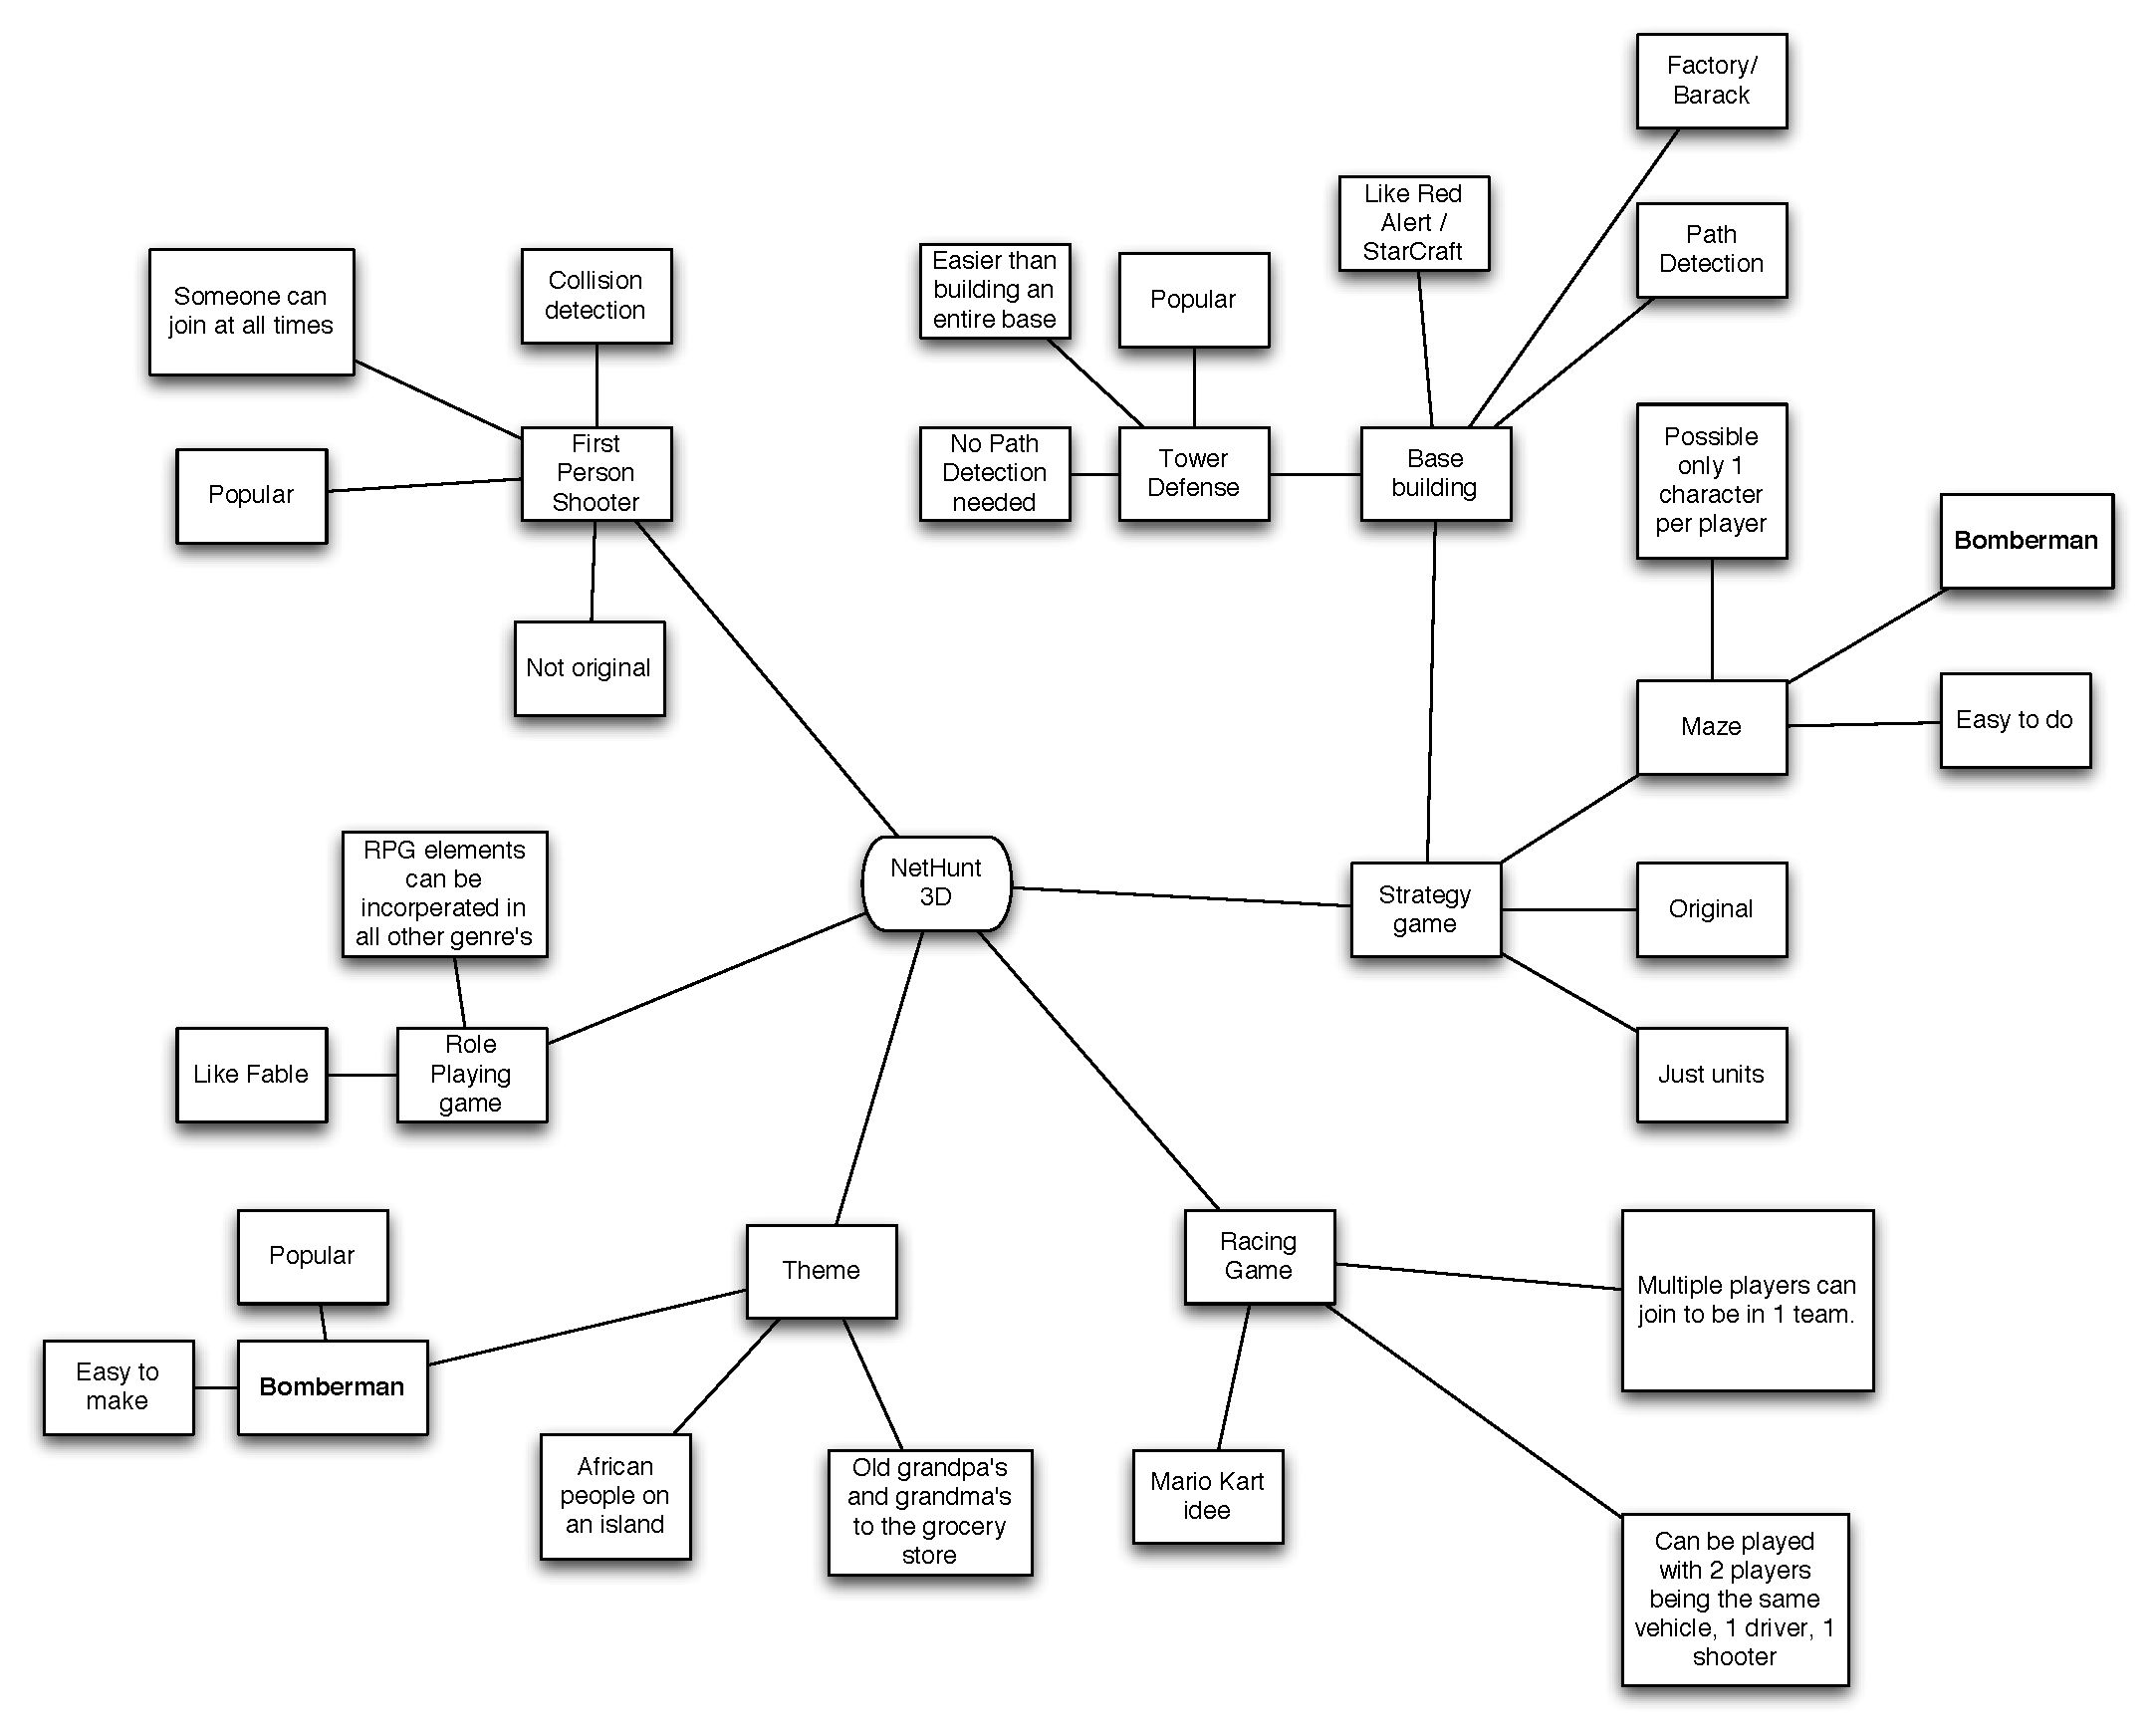
\includegraphics[width=\textwidth]{mindmap}

We started this project with a brainstorming session. We wrote all our ideas down on a whiteboard and selected parts that we did and did not like. We eventually ended up with a Bomberman-themed game with strategic elements (exploring a maze, controlling an area) and shooter elements (action-orientation, fierce competition).

We decided on this formula because the basics are familiar, making for relatively straightforward implementation and because it has a popular and fast kind of gameplay with a low barrier to entry. Also, bombing and powerups (see also: \ref{cha:defs}) allow us to give the game a unique look and feel.


\chapter{Gameplay}
This description of the gameplay is based on the `should have' version of the game. The game is similar to bomberman. Players, represented by avatars (see also: \ref{cha:defs}), spawn (see also: \ref{cha:defs}) in a level (see also: \ref{cha:defs}). They have a starting score, number of bombs and bomb power. They can move continuously (see also: \ref{cha:defs}) through a mazelike environment. Of course, players can not move through the walls of the maze, nor can they move through other players' avatars or bombs. The walls are made of two types, walls which can and walls which can not be blown up by bombs. The number of bombs denotes the amount of bombs which can be placed simultaneously on the map. When a bomb of a player explodes, the player can place an extra bomb again.

Player interaction occurs mainly through `bombing': players can have a number of bombs at any one time, which they can leave anywhere in the maze. These bombs explode after a while, hitting anyone who is too close, what constitutes `too close' being determined by the power of a player's bombs. Players can gain extra bombs and bomb power through finding powerups, which are located inside the walls of the games. When a certain wall is blown up, the powerup appears. *NOTE: not all walls contain powerups, they are scattered randomly. Some may convey another bonus, if we can find the time to implement that.

If players are hit, they are removed from the level and must wait for the next round. When only one player is left, that player has won the round. Each round has a time limit in which players can try to survive. When the clock has reached zero, the player with the most powerups wins. The players' scores are kept throughout multiple games, showing their ranking in the ongoing competition.

\chapter{Interface}
The players have a first person view (see also: \ref{cha:defs}) of the level, which takes up most of the screen. The other players' avatars and the level are shown in 3D, but the level is essentially 2D, that is, it can be described by a 2D map.

The players' number of bombs, their power and any special powerups are all displayed in the game window, which also contains a minimap (see also: \ref{cha:defs}) showing the player's environment.

The graphical theme will be similar to bomberman's: cartoony and futuristic. This theme will not influence the game's implementation until much later in the project, however and the specifics are not set in stone. We expect our ideas about the theme to evolve as we continue working on the project.

Players use a combination of the mouse and keyboard to control their movements: they move the mouse to turn, click mouse buttons to perform basic actions (place bombs), use the arrow keys to move and sidestep and the other keyboard buttons for any special moves and actions which might be implemented.

\chapter{Winning the game}
The main goal of the game (varying slightly between game modes) is being the last man standing in most rounds.

We might include the option to play the game in different modes, in which the objectives vary, if we have time. Inspiration on that matter can easily be drawn from so called `shooter' games and these modes may include:

\begin{itemize}
  \item Deathmatch, in which the objective is doing as much bombing of others as possible within limited time or within a limited number of respawns.

  \item Capture the flag, in which the players are divided into teams and the objective is to steal the other team's `flag'-powerup from their base and run back to your own.

  \item Greed, in which the player who gathers most powerups wins.
\end{itemize}

\chapter{The features}

\section{Must have} % (fold)
\label{sec:must_have}
The game must have these features.

 \begin{itemize}
  \item Collision detection
  \item A map to play on
  \item Network functionality
  \item An interface
  \item Powerups
 \end{itemize}
% section must_have (end)

\section{Ought to have} % (fold)
\label{sec:ought_to_have}
The game ought to have these features to conform to reasonable expectations.

\begin{itemize}
  \item Weapons
  \item Audio
\end{itemize}
% section ought_have (end)

\section{Should have} % (fold)
\label{sec:should_have}
The game should have these features, they are feasible and improve it greatly.

\begin{itemize}
  \item Chatting
  \item Multiple maps
  \item Multiple avatar textures
\end{itemize}
% section should_have (end)

\section{Could have} % (fold)
\label{sec:could_have}
We might include these features, so we should design the game so that we can add them later.

\begin{itemize}
  \item A map editor
  \item Game rules (for mods)
  \item Different game modes
  \item Intro/victory/scenario movies
\end{itemize}
% section could_have (end)

\section{Want to have} % (fold)
\label{sec:want_to_have}
If we have a lot of extra time, these are the features we want to add to the game.

\begin{itemize}
  \item Dynamics
  \item Physics
  \item No copyright material / Own copyright material
\end{itemize}
% section want_have (end)

\chapter{Technological}

We will use a star-network for communication between the players. For the graphics we will use Python and OpenGL with the PyOpenGL package for binding them. We will also use the PyGame library for some auxiliary functions, though we will still have to do the main graphics programming ourselves, as PyGame only helps with 2D graphics.

The program will consist of several components: a main component which handles the graphics and the game state, one for the network and one to handle user input.

\end{document}
